\documentclass[11pt,a4paper]{article}

\usepackage[margin=1in]{geometry}
\usepackage{amsmath,amssymb,bm}
\usepackage{graphicx}
\usepackage{booktabs}
\usepackage{hyperref}
\usepackage{xcolor}

\hypersetup{
  colorlinks=true,
  linkcolor=blue!50!black,
  citecolor=blue!50!black,
  urlcolor=blue!50!black,
}

% Float placement: keep results figures with Section~4
\renewcommand{\topfraction}{0.9}
\renewcommand{\bottomfraction}{0.8}
\renewcommand{\textfraction}{0.07}
\renewcommand{\floatpagefraction}{0.75}
\setcounter{topnumber}{4}
\setcounter{bottomnumber}{3}
\setcounter{totalnumber}{6}

% Prefer figures/paper/ (compressed rasters) before the full-resolution archive.
\graphicspath{{../figures/paper/}{figures/paper/}{../figures/}{figures/}}

\newcommand{\Nside}{N_{\mathrm{side}}}
\newcommand{\uK}{\,\mu\mathrm{K}}
\newcommand{\GHz}{\,\mathrm{GHz}}
\newcommand{\qopt}{q_{\mathrm{opt}}}
\newcommand{\qtrue}{q_{\mathrm{true}}}

\title{%
  Multi-frequency synthetic CMB skies from FLAMINGO lightcones:\\
  construction, spectral validation, and tests of ILC and\\
  matched-filter cluster finding
}

\author{%
  L.~Xu and collaborators
}

\date{\today}

\begin{document}
\maketitle

\begin{abstract}
We construct full-sky, multi-frequency synthetic millimetre skies from the
FLAMINGO hydrodynamical lightcones of Yang et~al., combining a lensed primary
cosmic microwave background (CMB) with thermal and kinetic Sunyaev--Zel'dovich
(tSZ, kSZ) anisotropies and the cosmic infrared background (CIB). All four
components share the same lightcone rotations, so their physical
cross-correlations are preserved. Maps are produced at native HEALPix resolution
$\Nside=4096$ in thermodynamic temperature for six Planck High Frequency
Instrument (HFI) channels. We specify the spectral kernels, unit conversions
and frequency extensions used for each component, and the deliberate omissions
(Galactic emission, radio sources, relativistic tSZ). Angular power spectra of
the secondary and foreground maps recover the CIB auto- and cross-spectra and
the $y$, kSZ and lensing auto-spectra reported by Yang et~al. Applying Planck
NPIPE noise and PR4 Galactic and point-source masks, we reconstruct Compton~$y$
with harmonic and needlet internal linear combination (ILC) and search for
galaxy clusters with multi-frequency matched filters in iterative (iMMF) and
spectrally constrained (sciMMF) modes. On a Planck-like footprint at detection
signal-to-noise $\qopt\ge 5$, both filters achieve purity $\approx 76$--$77\%$
and completeness $\approx 77\%$ relative to fixed-template matched-filter truth.
The mocks provide a controlled, extragalactic laboratory in which algorithm
performance can be judged against known $y$ and known clusters under realistic
Planck noise and masking.
\end{abstract}

\tableofcontents
\newpage

%==============================================================================
\section{Introduction}
\label{sec:intro}
%==============================================================================

Precision tests of component separation and cluster detection at millimetre
wavelengths require simulations in which the primary CMB, secondary anisotropies
and extragalactic foregrounds are correlated as in the real Universe, yet the
true Compton-$y$ field and cluster population remain known. Hydrodynamical
simulations that integrate tSZ, kSZ, CMB lensing and infrared emission along a
common lightcone satisfy this requirement. The FLAMINGO project has released
full-sky maps of these quantities from a large cosmological volume
\cite{Yang:2026flamingo}, providing the physical ingredients for end-to-end
Planck-like analyses.

This work builds multi-frequency temperature skies from those lightcones and
uses them for two canonical applications. First, we form coadded maps with
Planck beams and NPIPE instrumental noise \cite{Planck:2020npipe} and reconstruct
Compton~$y$ with needlet and harmonic internal linear combination (ILC) methods
following McCarthy \& Hill \cite{McCarthyHill:2024}. Second, we apply
multi-frequency matched filters---the iterative matched multi-filter (iMMF) and
the spectrally constrained iMMF (sciMMF) of Zubeldia et~al.\
\cite{Zubeldia:2023a,Zubeldia:2023b}---to produce cluster catalogues at
detection threshold $\qopt\ge 5$, and measure purity and completeness against
fixed-template truth signal-to-noise on the same footprint.

The sky model is intentionally minimal: lensed primary CMB, non-relativistic
tSZ, kSZ and CIB, with no Galactic dust, synchrotron or free--free and no radio
point sources. That choice isolates extragalactic contamination and
instrumental noise as the limiting factors for SZ science, at the cost of
understating foreground complexity at $545$ and $857\GHz$ relative to flight
data. Section~\ref{sec:data} summarises the FLAMINGO inputs.
Section~\ref{sec:methods} details the construction of multi-frequency
temperature maps. Section~\ref{sec:results} presents power-spectrum validation
and the ILC and cluster-finding results. Section~\ref{sec:conclusions} states
our conclusions.

%==============================================================================
\section{FLAMINGO lightcone inputs}
\label{sec:data}
%==============================================================================

\subsection{Simulation and map products}
\label{sec:flamingo}

We use the flagship FLAMINGO run \texttt{L2800N5040} (\texttt{L2p8\_m9}): a
comoving box of side $2.8\,h^{-1}\mathrm{Gpc}$ with $5040^3$ particles per
species, intermediate mass resolution $m_9$, and the \texttt{HYDRO\_FIDUCIAL}
feedback calibration in a DES Year~3 $3\times2$pt+external $\Lambda$CDM cosmology
\cite{Yang:2026flamingo}. Lightcone shells are stacked with common random
rotations every box length so that cross-correlations among Compton~$y$, kSZ,
lensing convergence $\kappa$ and CIB are preserved. Maps are HEALPix
RING-ordered float32 fields at $\Nside=4096$ (pixel scale $\approx 0.86'$) in
Galactic coordinates. Unless noted, we analyse a single observer
(\texttt{lightcone0}).

The fields used here are:
\begin{itemize}
  \item lensed Compton~$y$ (dimensionless);
  \item lensed Doppler~$b$, related to the kSZ temperature by
    $\Delta T_{\mathrm{kSZ}}/T_{\mathrm{CMB}}=-b$;
  \item CMB lensing convergence $\kappa$;
  \item bandpass-integrated CIB intensity at $217$, $353$, $545$ and $857\GHz$
    in $\mathrm{Jy\,sr^{-1}}$, for the fiducial three-parameter dust model.
\end{itemize}
Secondary maps are already lensed shell-by-shell with the cumulative $\kappa$
field \cite{Yang:2026flamingo}. The cosmology adopted for the primary CMB matches
Table~1 of Yang et~al.:
\begin{equation}
  h=0.681,\;
  \Omega_{\mathrm{m}}=0.306,\;
  \Omega_{\mathrm{b}}=0.0486,\;
  m_\nu=0.06\,\mathrm{eV},\;
  A_{\mathrm{s}}=2.099\times10^{-9},\;
  n_{\mathrm{s}}=0.967.
\end{equation}
We use $T_{\mathrm{CMB}}=2.7255\,\mathrm{K}$ consistently for all spectral
conversions.

\subsection{Scope of the mock sky}
\label{sec:sky-model-scope}

The additive sky model has exactly four components,
\begin{equation}
  \label{eq:sky}
  \Delta T(\hat n,\nu)
  =
  \Delta T_{\mathrm{CMB}}(\hat n)
  +
  \Delta T_{\mathrm{tSZ}}(\hat n,\nu)
  +
  \Delta T_{\mathrm{kSZ}}(\hat n)
  +
  \Delta T_{\mathrm{CIB}}(\hat n,\nu),
\end{equation}
all expressed in thermodynamic $\mu\mathrm{K}_{\mathrm{CMB}}$ after spectral
conversion. We deliberately exclude:
\begin{itemize}
  \item Galactic emission (thermal dust, synchrotron, free--free);
  \item radio point sources present in the FLAMINGO release;
  \item relativistic tSZ corrections;
  \item star-formation-rate maps as an additive temperature term (they are
    precursors of the CIB, not a separate sky component);
  \item $\kappa$ as a temperature term ($\kappa$ enters only through lensing of
    the primary CMB; secondary maps are already lensed upstream).
\end{itemize}
Instrumental noise is not baked into the component maps; it is added at analysis
time from official Planck NPIPE residual realisations
\cite{Planck:2020npipe}. Halo lightcone catalogues provide truth positions,
redshifts and masses for cluster validation.

%==============================================================================
\section{Construction of multi-frequency temperature maps}
\label{sec:methods}
%==============================================================================

\subsection{Primary CMB and lensing}
\label{sec:cmb}

An unlensed Gaussian temperature realisation is drawn from the unlensed scalar
$C_\ell^{TT}$ spectrum computed with CAMB \cite{Lewis:2000camb} at the FLAMINGO
cosmology (units $\mu\mathrm{K}^2$). The FLAMINGO $\kappa$ map is mean-subtracted
and converted to lensing-potential harmonics,
\begin{equation}
  \phi_{\ell m}
  =
  \frac{2}{\ell(\ell+1)}\,\kappa_{\ell m}
  \qquad (\ell\ge 2),
\end{equation}
with monopole and dipole of $\phi$ set to zero. Deflection is performed on a
full-sky CAR grid at resolution $\pi/(2\Nside)$ and reprojected to HEALPix. The
result is a lensed primary CMB map at $\Nside=4096$ in $\mu\mathrm{K}_{\mathrm{CMB}}$.

\subsection{Thermal Sunyaev--Zel'dovich effect}
\label{sec:tsz}

Given the lensed Compton-$y$ map, the non-relativistic thermodynamic temperature
at frequency $\nu$ is
\begin{equation}
  \label{eq:tsz}
  \Delta T_{\mathrm{tSZ}}(\nu)
  =
  T_{\mathrm{CMB}}\, y\, f(x),
  \qquad
  x=\frac{h\nu}{k_{\mathrm{B}}T_{\mathrm{CMB}}},
  \qquad
  f(x)=x\coth\!\left(\frac{x}{2}\right)-4.
\end{equation}
We evaluate Equation~\eqref{eq:tsz} at the six Planck HFI frequencies
$\{100,143,217,353,545,857\}\GHz$. The dimensionless $y$ map is retained as
ground truth for ILC and cluster studies.

\subsection{Kinetic Sunyaev--Zel'dovich effect}
\label{sec:ksz}

In thermodynamic units the kSZ is frequency-independent:
\begin{equation}
  \label{eq:ksz}
  \Delta T_{\mathrm{kSZ}}
  =
  -T_{\mathrm{CMB}}\, b.
\end{equation}
A single $\Delta T$ map therefore serves all channels.

\subsection{Cosmic infrared background}
\label{sec:cib}

Released CIB maps at $217$, $353$, $545$ and $857\GHz$ are bandpass-convolved
specific intensities $I_\nu$ in $\mathrm{Jy\,sr^{-1}}$. Conversion to
thermodynamic temperature uses
\begin{equation}
  \Delta T_{\mathrm{CIB}}(\nu)
  =
  \frac{I_\nu}{\mathrm{d}B_\nu/\mathrm{d}T\big|_{T_{\mathrm{CMB}}}}
  \times 10^{6}\,\uK.
\end{equation}
Frequencies outside the released set are approximated as follows
\cite{Yang:2026flamingo}: exact released bands are used unchanged; intermediate
frequencies use logarithmic interpolation in $I_\nu$; frequencies below
$217\GHz$ (including $100$ and $143\GHz$) are scaled from the nearest released
band with the three-parameter greybody SED at effective redshift
$z_{\mathrm{eff}}=1.5$,
\begin{equation}
  \Theta(\nu,T_{\mathrm{d}})
  \propto
  \frac{\nu^{\beta_{\mathrm{d}}+3}}{e^{h\nu/k_{\mathrm{B}}T_{\mathrm{d}}}-1},
  \qquad
  T_{\mathrm{d}}(z)=T_0(1+z)^{\alpha},
\end{equation}
with $\beta_{\mathrm{d}}=1.65$, $T_0=35.14\,\mathrm{K}$ and $\alpha=0$. This
approximation neglects frequency decorrelation of small-scale structure, which is
acceptable where the CIB is subdominant to the CMB and instrumental noise.

\subsection{Beams, noise and masks}
\label{sec:beams-noise}

\paragraph{Beams.}
Planck HFI Gaussian full-width half-maxima (instrument paper Table~I) are
$\{9.66',7.22',4.90',4.92',4.67',4.22'\}$ at
$\{100,143,217,353,545,857\}\GHz$. Component products are stored
beam-unconvolved; beams are applied when forming total skies for ILC and matched
filters.

\paragraph{Noise.}
Planck NPIPE noise Monte Carlos are end-to-end residual maps (pipeline output
minus input), HEALPix $\Nside=2048$, full sky, anisotropic and position-tied
\cite{Planck:2020npipe}. Channels at $100$--$353\GHz$ are in
$\mathrm{K}_{\mathrm{CMB}}$; $545$ and $857\GHz$ are in $\mathrm{MJy\,sr^{-1}}$
and require conversion through $\mathrm{d}B_\nu/\mathrm{d}T$. Independently
destriped detector-set splits A and B provide noise-decoupled cross-spectra.
Noise must not be rotated relative to the signal.

\paragraph{Masks.}
PR4 NILC multi-field masks supply a soft Galactic plane cut and binary
point-source holes. Analyses use a binary $\mathrm{GAL}\times\mathrm{PS}$
product at $\Nside=2048$. Matched-filter tiling further apodises flat-sky
galaxy, point-source and tile-boundary masks.

\subsection{Analysis applications}
\label{sec:downstream}

\paragraph{ILC Compton-$y$ reconstruction.}
Multi-frequency coadds (Equation~\ref{eq:sky}) are beam-smoothed, downgraded to
$\Nside=2048$ and combined with NPIPE splits. Harmonic ILC (HILC) and needlet
ILC (NILC) preserve the tSZ spectral response, optionally deprojecting CMB
and/or CIB \cite{McCarthyHill:2024}. Spectra are reported after deconvolution of
the common $5'$ working beam for comparison with beam-free truth $y$.

\paragraph{Matched-filter cluster finding.}
SZiFi implements iterative multi-frequency matched filters (iMMF) and
spectrally constrained filters that null a CIB spectral template (sciMMF)
\cite{Zubeldia:2023a,Zubeldia:2023b}. The sky is analysed in $14.8^\circ$ tiles
with NPIPE noise and PR4 masks; catalogues are thresholded at $\qopt>5$. Truth
signal-to-noise for completeness uses a fixed-template matched filter on the
known $y$ field within the same footprint and redshift cut.

%==============================================================================
\section{Results}
\label{sec:results}
%==============================================================================

\subsection{Component maps}
\label{sec:component-maps}

Figure~\ref{fig:overview} shows the four components at $353\GHz$.
Figure~\ref{fig:cmb-y} highlights the lensed primary CMB and the full-sky
Compton-$y$ field. Frequency dependence of tSZ and CIB is shown in
Figures~\ref{fig:tsz-freq} and~\ref{fig:cib-freq}. The maps exhibit the expected
morphology: acoustic structure in the CMB, cluster-scale peaks in $y$, a diffuse
kSZ pattern, and dusty large-scale structure in the CIB that brightens toward
higher frequencies.

\begin{figure}[htbp]
  \centering
  
\includegraphics[width=\textwidth]{components_overview_353GHz_mollview.jpg}
  \caption{Four-component sky model at $353\GHz$ (Mollweide, Galactic
    coordinates, $\Nside=4096$). Clockwise from top-left: lensed primary CMB,
    tSZ $\Delta T$, kSZ $\Delta T$, and CIB $\Delta T$ (all temperatures in
    $\mu\mathrm{K}_{\mathrm{CMB}}$).}
  \label{fig:overview}
\end{figure}

\begin{figure}[htbp]
  \centering
  
\includegraphics[width=0.49\textwidth]{components_cmb_lensed_mollview.jpg}
  \hfill
  
\includegraphics[width=0.49\textwidth]{components_tsz_compton_y_mollview.jpg}
  \caption{Lensed primary CMB (left; $\mu\mathrm{K}_{\mathrm{CMB}}$) and
    Compton-$y$ ground truth (right).}
  \label{fig:cmb-y}
\end{figure}

\begin{figure}[htbp]
  \centering
  
\includegraphics[width=\textwidth]{components_tsz_deltaT_allfreq_mollview.jpg}
  \caption{tSZ thermodynamic temperature at the six Planck HFI frequencies
    (Equation~\ref{eq:tsz}). The spectral null near $217\GHz$ and the sign change
    across it are visible.}
  \label{fig:tsz-freq}
\end{figure}

\begin{figure}[htbp]
  \centering
  
\includegraphics[width=\textwidth]{components_cib_deltaT_allfreq_mollview.jpg}
  \caption{CIB in $\mu\mathrm{K}_{\mathrm{CMB}}$ after conversion from released
    intensity maps, with greybody SED scaling at $100$ and $143\GHz$.}
  \label{fig:cib-freq}
\end{figure}

\subsection{Power-spectrum validation}
\label{sec:pspec}

We recompute angular power spectra of the native-resolution integrated maps with
monopole subtraction and HEALPix pixel-window deconvolution. Multipoles are
binned with $\Delta\ell=7$ following Yang et~al.

Figure~\ref{fig:cib-auto} shows CIB auto-spectra at $217$--$857\GHz$.
Figure~\ref{fig:cib-decorr} reports the mean frequency decorrelation
\begin{equation}
  r_{\nu\nu'}
  =
  \frac{C_\ell^{\nu\times\nu'}}
       {\sqrt{C_\ell^{\nu\nu}\,C_\ell^{\nu'\nu'}}}
\end{equation}
averaged over $150<\ell<1000$, reproducing the structure of Yang et~al.\ Table~3:
strong correlation among neighbouring bands and progressive loss of coherence
between $217$ and $857\GHz$. Figure~\ref{fig:cib-cross} shows CIB$\times y$ and
CIB$\times\kappa$ cross-spectra. Figure~\ref{fig:autos} shows the Compton-$y$,
kSZ (thermodynamic) and $\kappa$ auto-spectra. These measurements confirm that
the lightcone products and unit conversions recover the published secondary and
foreground statistics at $\Nside=4096$.

\begin{figure}[htbp]
  \centering
  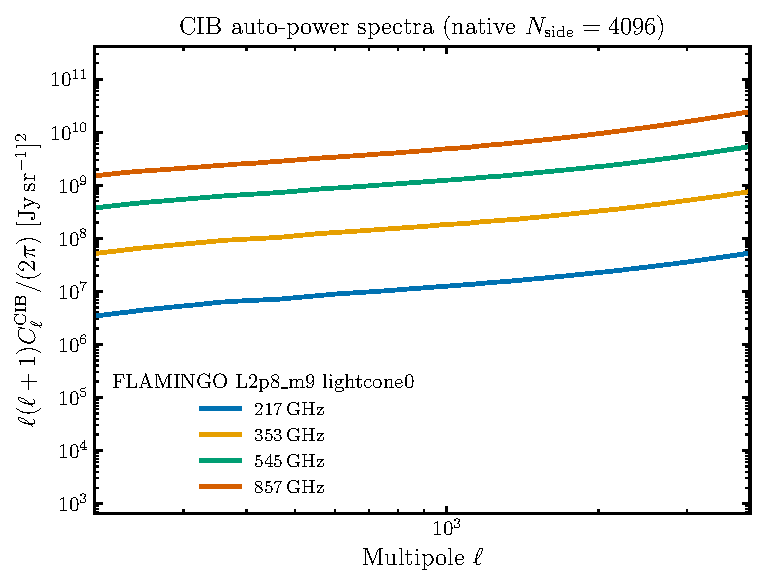
\includegraphics[width=0.88\textwidth]{yang26_fig8left_cib_auto_spectra.pdf}
  \caption{CIB auto-power spectra at $\Nside=4096$ (cf.\ Yang et~al.\ Fig.~8,
    left).}
  \label{fig:cib-auto}
\end{figure}

\begin{figure}[htbp]
  \centering
  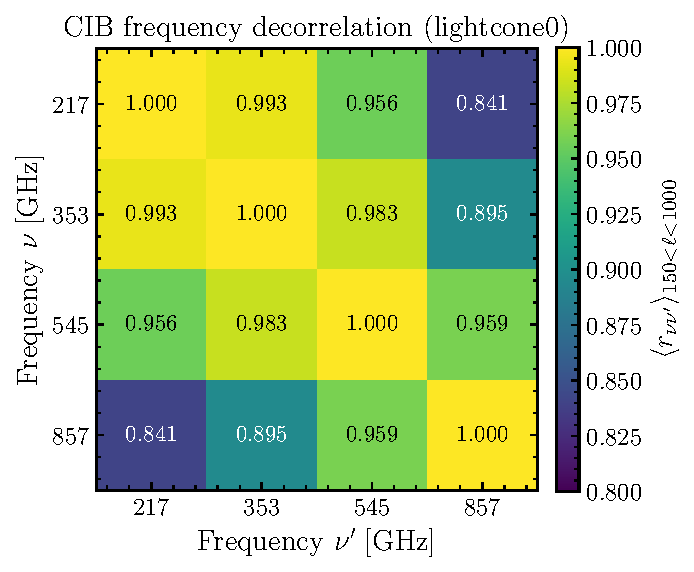
\includegraphics[width=0.72\textwidth]{yang26_table3_cib_decorrelation.pdf}
  \caption{Mean CIB frequency decorrelation $\langle r_{\nu\nu'}\rangle$ for
    $150<\ell<1000$ (cf.\ Yang et~al.\ Table~3).}
  \label{fig:cib-decorr}
\end{figure}

\begin{figure}[htbp]
  \centering
  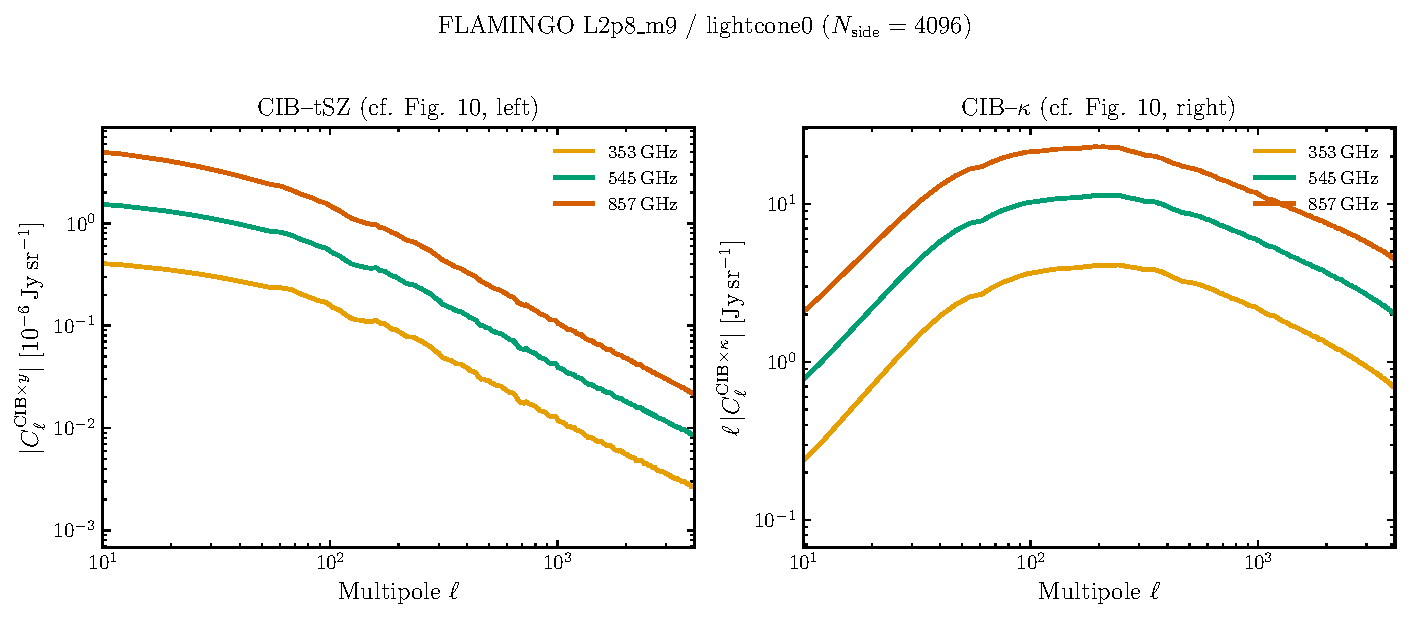
\includegraphics[width=0.95\textwidth]{yang26_fig10_cib_tsz_kappa_cross.pdf}
  \caption{Absolute CIB$\times y$ (left) and
    $\ell\,|C_\ell^{\mathrm{CIB}\times\kappa}|$ (right) at $353$, $545$ and
    $857\GHz$ (cf.\ Yang et~al.\ Fig.~10).}
  \label{fig:cib-cross}
\end{figure}

\begin{figure}[htbp]
  \centering
  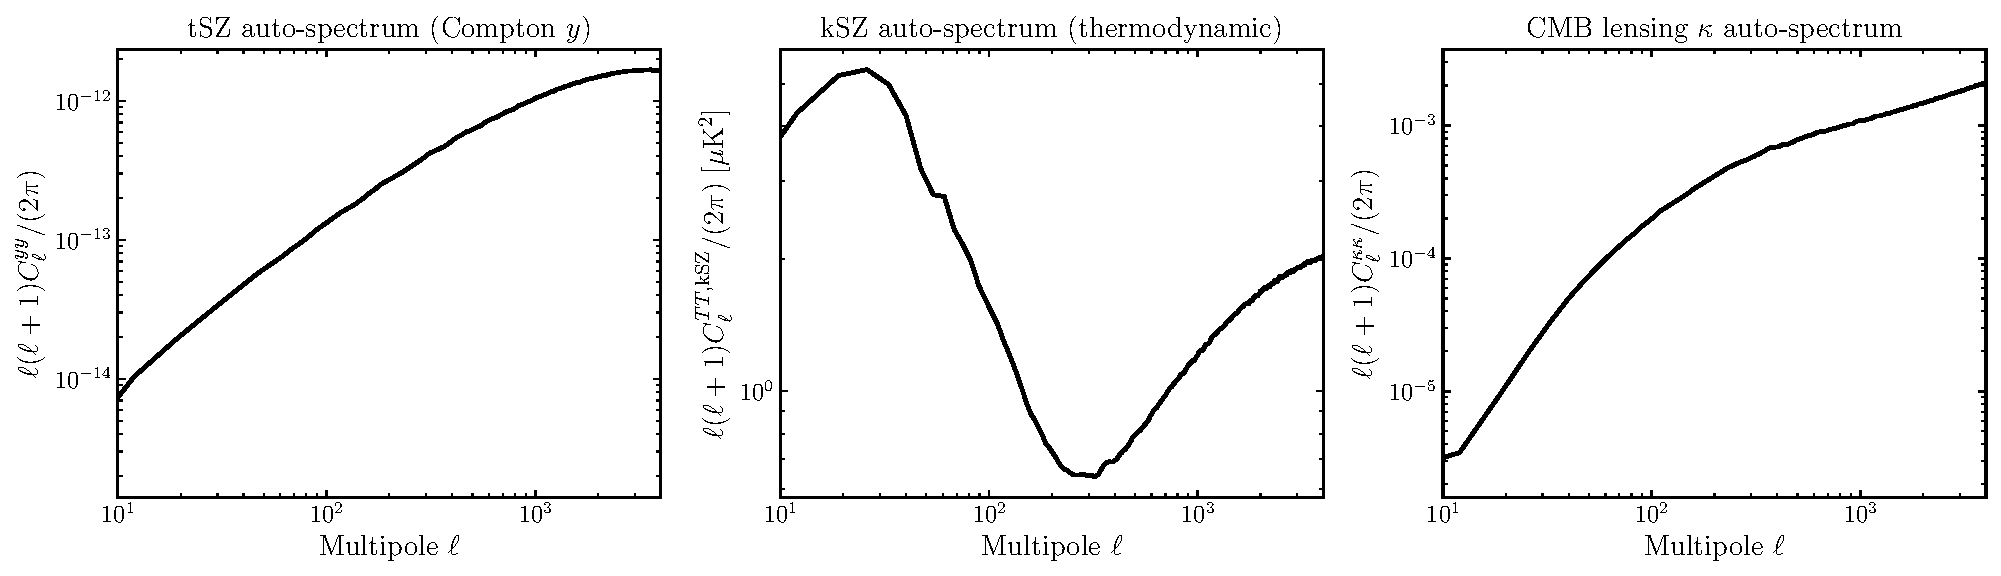
\includegraphics[width=0.98\textwidth]{yang26_figs67_tsz_ksz_kappa_autos.pdf}
  \caption{Auto-spectra of Compton~$y$ (left), kSZ thermodynamic temperature
    (centre) and CMB lensing $\kappa$ (right) at native resolution.}
  \label{fig:autos}
\end{figure}

\subsection{Instrumental noise}
\label{sec:noise-results}

Figure~\ref{fig:noise} shows NPIPE detector-set A residual maps at
$100$--$353\GHz$ for one Monte Carlo realisation. Depth varies strongly across
the sky (ecliptic-plane striping and polar deep fields), which motivates
split-based cross-spectra and footprint cuts in both ILC and cluster finding.

\begin{figure}[htbp]
  \centering
  
\includegraphics[width=0.92\textwidth]{planck_noise_gallery_mc00200.jpg}
  \caption{Planck NPIPE noise realisation \texttt{mc\_00200}, detector-set A, at
    $100$, $143$, $217$ and $353\GHz$ ($\mu\mathrm{K}_{\mathrm{CMB}}$).}
  \label{fig:noise}
\end{figure}

\subsection{ILC reconstruction of Compton-$y$}
\label{sec:ilc}

\subsubsection{Baseline HILC and NILC}

Figure~\ref{fig:ilc-spectra} compares the truth $y$ auto-spectrum with
beam-deconvolved HILC ($A\times B$) and NILC reconstructions on coadds that
include NPIPE noise. Figure~\ref{fig:ilc-transfer} shows the transfer
$T_\ell=C_\ell^{y_{\mathrm{ILC}}\times y_{\mathrm{true}}}/C_\ell^{yy}$. Both
methods recover the large-scale $y$ power; residuals at high multipoles reflect
noise and residual foregrounds after beam deconvolution.

\begin{figure}[htbp]
  \centering
  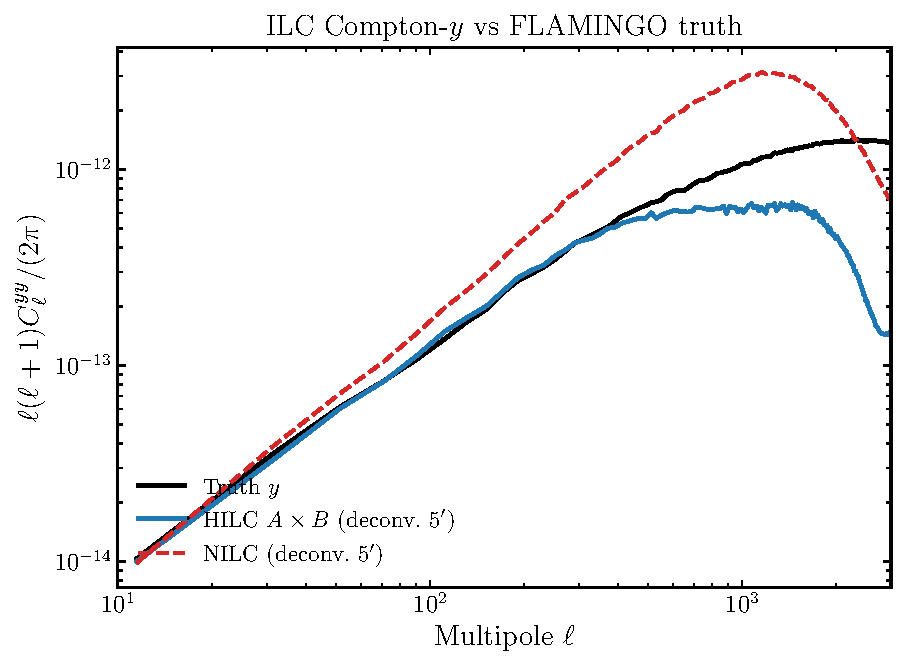
\includegraphics[width=\textwidth]{ilc_y_vs_truth_spectra_pub.pdf}
  \caption{Beam-deconvolved Compton-$y$ power spectra: FLAMINGO truth versus HILC
    (split $A\times B$) and NILC on mock skies with NPIPE noise.}
  \label{fig:ilc-spectra}
\end{figure}

\begin{figure}[htbp]
  \centering
  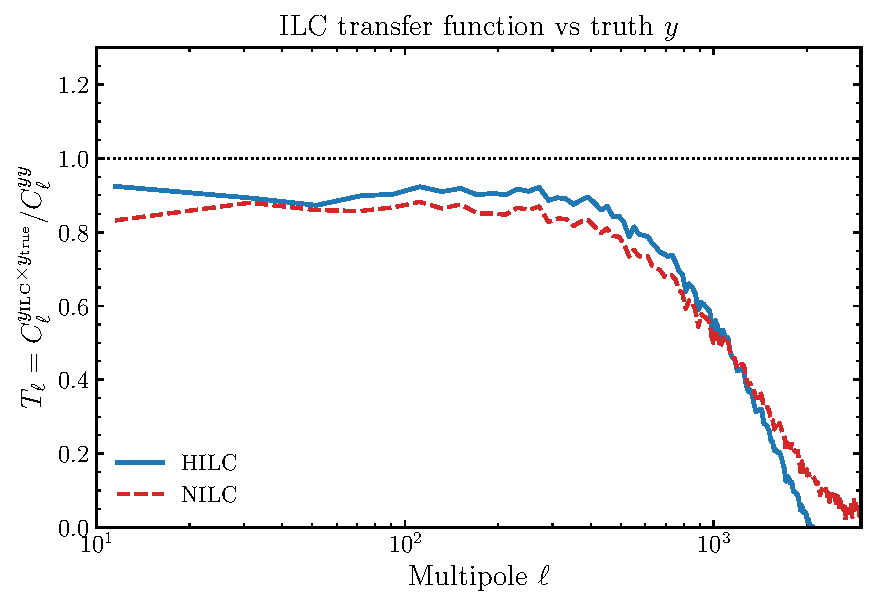
\includegraphics[width=\textwidth]{ilc_transfer_vs_truth_pub.pdf}
  \caption{ILC transfer function relative to truth $y$ for HILC and NILC.}
  \label{fig:ilc-transfer}
\end{figure}

\subsubsection{Constrained ILC deprojection suite}
\label{sec:ilc-deproj}

Following McCarthy \& Hill \cite{McCarthyHill:2024}, we run a suite of
\emph{constrained} (deprojected) HILC reconstructions that preserve unit
response to tSZ while nulling one or more foreground spectral energy
distributions (SEDs). With six HFI channels the available options include
nulling the CMB blackbody, a modified-blackbody CIB template, and first-order
CIB SED derivatives with respect to spectral index ($\delta\beta$) and dust
temperature ($\delta T$). The mock sky contains CMB, tSZ, kSZ and CIB only, so
CIB deprojection is the primary science-motivated constraint; CMB deprojection
also removes the thermodynamic kSZ because the two share a blackbody SED in
$\mu\mathrm{K}_{\mathrm{CMB}}$.

Table~\ref{tab:deproj} summarises validation metrics against the beam-convolved
truth $y$ map: map standard deviation $\sigma_y$, full-sky correlation after
common-beam matching, mid-$\ell$ correlation $\rho_{50\text{--}500}$, and a
mid-$\ell$ transfer estimate $T_{\mathrm{mid}}$.
Figure~\ref{fig:deproj-metrics} visualises the same suite;
Figure~\ref{fig:deproj-cl} shows auto-power spectra for selected deprojections.

\begin{table}[htbp]
  \centering
  \caption{HILC constrained-ILC deprojection suite (NPIPE split A) versus truth
    Compton-$y$. Mild CIB deprojection improves mid-$\ell$ correlation and
    transfer; multi-moment CIB constraints ($\delta\beta+\delta T$) inflate the
    residual variance by a factor of $\sim 2$--$3$ and destroy correlation with
    truth.}
  \label{tab:deproj}
  \begin{tabular}{lcccc}
    \toprule
    Deprojection & $\sigma_y$ & corr (beamed) & $\rho_{50\text{--}500}$ & $T_{\mathrm{mid}}$ \\
    \midrule
    None & $1.81\times10^{-6}$ & 0.473 & 0.654 & 0.909 \\
    CMB & $1.82\times10^{-6}$ & 0.470 & 0.655 & 0.910 \\
    CIB & $1.84\times10^{-6}$ & 0.496 & 0.671 & 0.960 \\
    CIB+CMB & $1.85\times10^{-6}$ & 0.493 & 0.672 & 0.959 \\
    CIB+$\delta\beta$ & $1.95\times10^{-6}$ & 0.463 & 0.614 & 0.949 \\
    CIB+$\delta\beta$+CMB & $1.97\times10^{-6}$ & 0.458 & 0.615 & 0.948 \\
    CIB+$\delta\beta$+$\delta T$ & $4.19\times10^{-6}$ & 0.226 & 0.279 & 1.000 \\
    CIB+$\delta\beta$+$\delta T$+CMB & $6.00\times10^{-6}$ & 0.159 & 0.271 & 0.995 \\
    \bottomrule
  \end{tabular}
\end{table}

\begin{figure}[htbp]
  \centering
  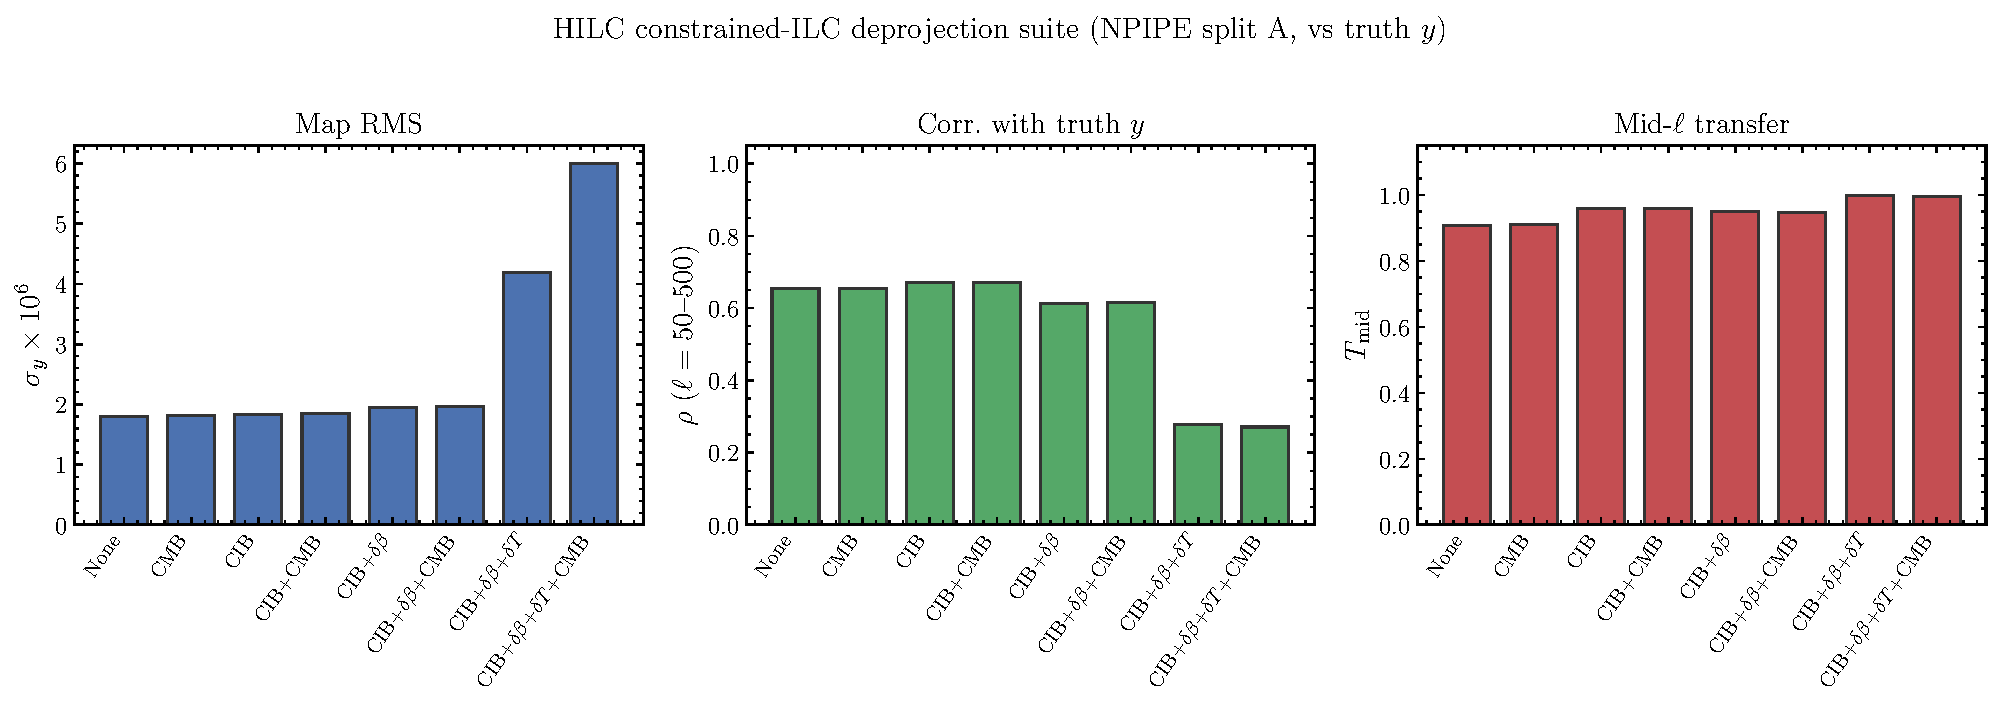
\includegraphics[width=\textwidth]{ilc_deproj_suite_metrics.pdf}
  \caption{HILC deprojection suite metrics versus truth $y$: map RMS (left),
    multipole-windowed correlation $\rho_{50\text{--}500}$ (centre), and
    mid-$\ell$ transfer (right).}
  \label{fig:deproj-metrics}
\end{figure}

\begin{figure}[htbp]
  \centering
  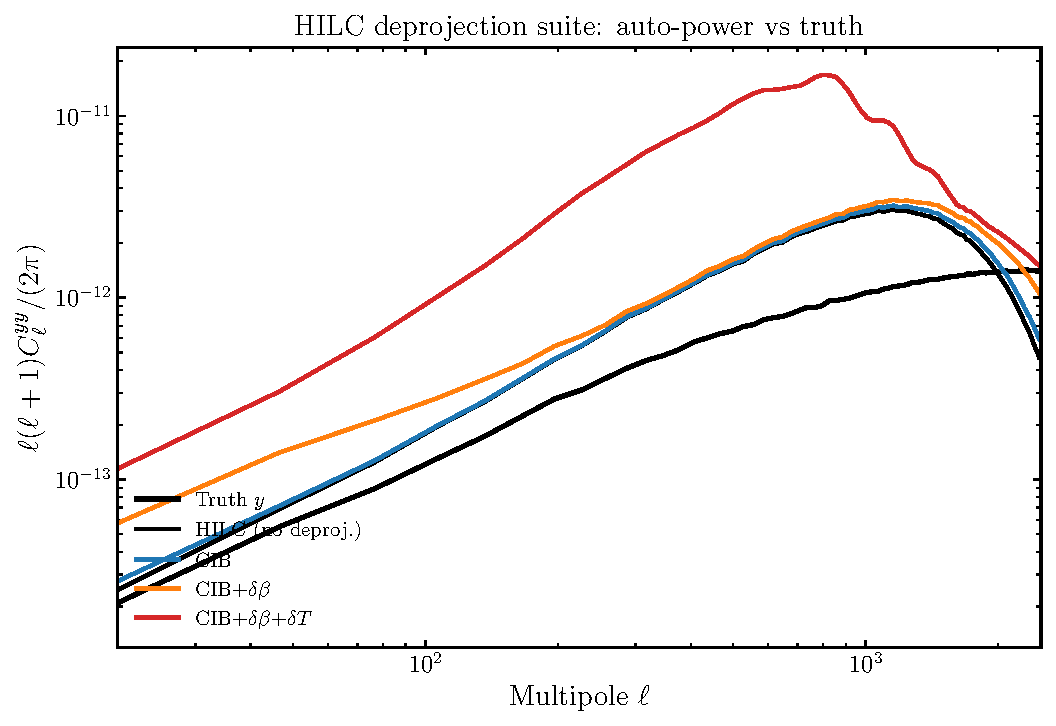
\includegraphics[width=\textwidth]{ilc_deproj_suite_autopower.pdf}
  \caption{Beam-deconvolved auto-power for selected HILC deprojections compared
    with truth $y$. CIB-only deprojection stays close to the unconstrained
    solution; adding $\delta\beta+\delta T$ moments raises small-scale power
    (noise penalty) by a large factor.}
  \label{fig:deproj-cl}
\end{figure}

The results encode a clear bias--noise trade-off. \textbf{CIB-only} deprojection
raises $\rho_{50\text{--}500}$ from $0.654$ to $0.671$ and $T_{\mathrm{mid}}$
from $0.909$ to $0.960$ with only a modest increase in $\sigma_y$. Adding CMB
to the constraint set leaves metrics essentially unchanged, as expected on a
mock without Galactic dust. First-order $\delta\beta$ deprojection already
reduces mid-$\ell$ correlation, and the full moment set
$\mathrm{CIB}+\delta\beta+\delta T$ (with or without CMB) more than doubles
$\sigma_y$ and collapses $\rho_{50\text{--}500}$ to $\sim 0.27$. On this
Galactic-free mock, therefore, mild CIB deprojection is beneficial for
correlation with truth $y$, whereas aggressive multi-moment constraints are
noise-dominated---consistent with the behaviour reported for Planck PR4 in
\cite{McCarthyHill:2024}.

\subsection{Matched-filter cluster catalogues}
\label{sec:szifi}

We run iMMF and sciMMF (CIB spectral constraint) on multi-frequency tiles with
NPIPE split A, PR4 $\mathrm{GAL}\times\mathrm{PS}$ masking, and catalogue
threshold $\qopt\ge 5$. Detections are matched to truth systems with
$\qtrue\ge 5$ (fixed-template matched filter on truth $y$) within $10'$,
restricted to $z\le 1$ and the unmasked footprint.

\subsubsection{Sky maps of found clusters}

Figure~\ref{fig:clusters-immf} shows all iMMF detections with $\qopt\ge 5$
overlaid on the truth Compton-$y$ map inside the PR4 footprint; circles scale
with the fitted $\theta_{500}$. Figure~\ref{fig:clusters-scimmf} is the
corresponding sciMMF catalogue. Figures~\ref{fig:tpfp-immf}
and~\ref{fig:tpfp-scimmf} colour the same detections by match outcome: lime
true positives and red false positives under the $10'$ Zubeldia-style match to
fixed-MMF truth. High-$q$ systems concentrate on bright $y$ peaks; residual
false positives include both threshold noise fluctuations and sources near the
matching boundary.

\begin{figure}[htbp]
  \centering
  
\includegraphics[width=\textwidth]{szifi_footprint_immf_mollview_detections.jpg}
  \caption{Truth Compton-$y$ (PR4 $\mathrm{GAL}\times\mathrm{PS}$ footprint)
    with iMMF detections at $\qopt\ge 5$ (cyan circles scaled by
    $\theta_{500}$).}
  \label{fig:clusters-immf}
\end{figure}

\begin{figure}[htbp]
  \centering
  
\includegraphics[width=\textwidth]{szifi_footprint_scimmf_mollview_detections.jpg}
  \caption{As Figure~\ref{fig:clusters-immf}, for sciMMF detections.}
  \label{fig:clusters-scimmf}
\end{figure}

\begin{figure}[htbp]
  \centering
  
\includegraphics[width=\textwidth]{szifi_footprint_immf_mollview_tp_fp.jpg}
  \caption{iMMF detections classified as true positives (lime) and false
    positives (red) after $10'$ matching to fixed-MMF $\qtrue\ge 5$ truth.}
  \label{fig:tpfp-immf}
\end{figure}

\begin{figure}[htbp]
  \centering
  
\includegraphics[width=\textwidth]{szifi_footprint_scimmf_mollview_tp_fp.jpg}
  \caption{As Figure~\ref{fig:tpfp-immf}, for sciMMF.}
  \label{fig:tpfp-scimmf}
\end{figure}

\subsubsection{Purity and completeness}

Table~\ref{tab:szifi} summarises the catalogues. Both methods achieve purity
($\approx 76$--$77\%$). Completeness relative to the fixed-MMF-detectable
truth sample is $\approx 77\%$ for both; sciMMF returns more detections (832
versus 731 after footprint cuts) at essentially the same purity.
Figure~\ref{fig:szifi-bench} shows purity and completeness summary bars
(completeness numerators count detectable truths that were found:
$333/430$ for iMMF and $334/430$ for sciMMF);
Figure~\ref{fig:szifi-snr} shows completeness versus truth SNR and purity versus
detection threshold; Figure~\ref{fig:szifi-compare} compares the two methods.
Completeness rises with truth SNR and approaches unity for the highest-$\qtrue$
systems, while purity improves as the detection threshold is raised above $q=5$.

\begin{table}[htbp]
  \centering
  \caption{SZiFi footprint catalogues (NPIPE split A, $\qopt\ge 5$, PR4
    $\mathrm{GAL}\times\mathrm{PS}$, match radius $10'$, $z\le 1$, truth =
    fixed-MMF $\qtrue\ge 5$). Completeness is
    $(N_{\mathrm{truth}}^{\mathrm{det.}}-N_{\mathrm{undetected}})/N_{\mathrm{truth}}^{\mathrm{det.}}$.}
  \label{tab:szifi}
  \begin{tabular}{lcccccc}
    \toprule
    Method & $N_{\mathrm{det}}$ & $N_{\mathrm{TP}}$ & $N_{\mathrm{FP}}$ &
    Purity & $N_{\mathrm{truth}}^{\mathrm{det.}}$ & Completeness \\
    \midrule
    iMMF   & 731 & 564 & 167 & 0.772 & 430 & 0.774 \\
    sciMMF & 832 & 633 & 199 & 0.761 & 430 & 0.777 \\
    \bottomrule
  \end{tabular}
\end{table}

\begin{figure}[htbp]
  \centering
  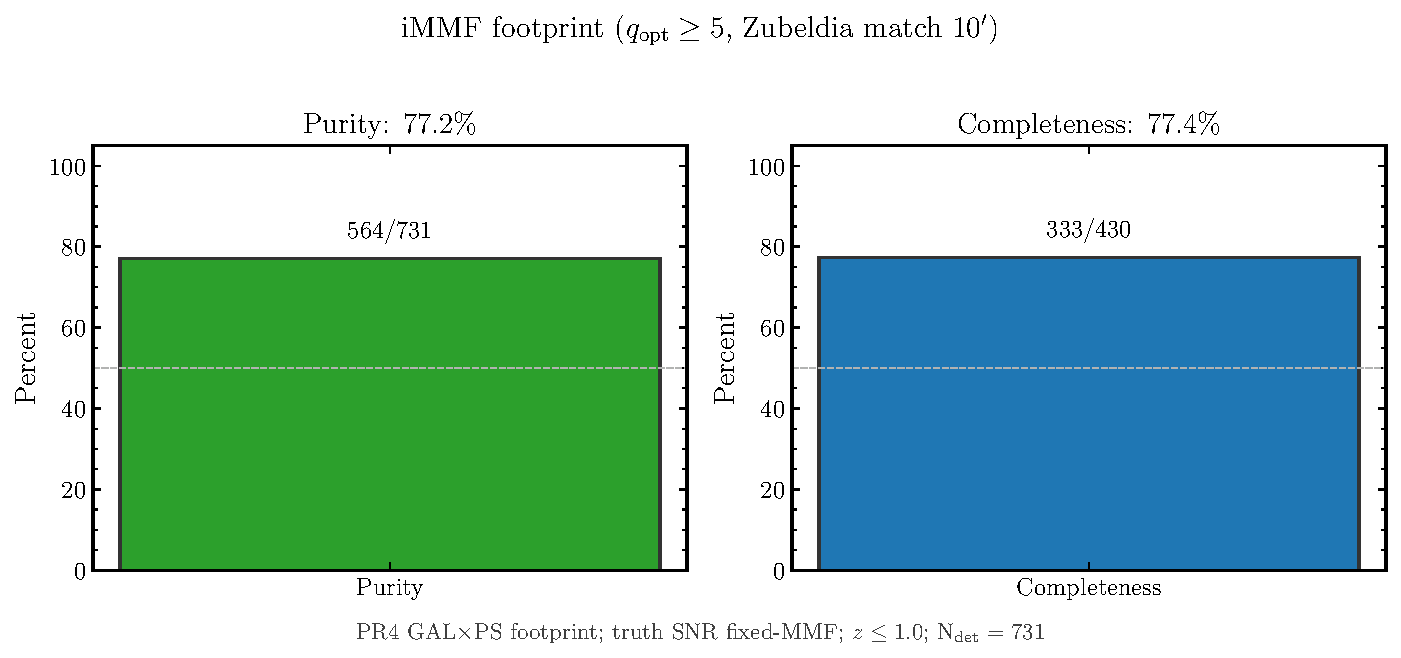
\includegraphics[width=0.49\textwidth]{szifi_footprint_immf_benchmark_szifi.pdf}
  \hfill
  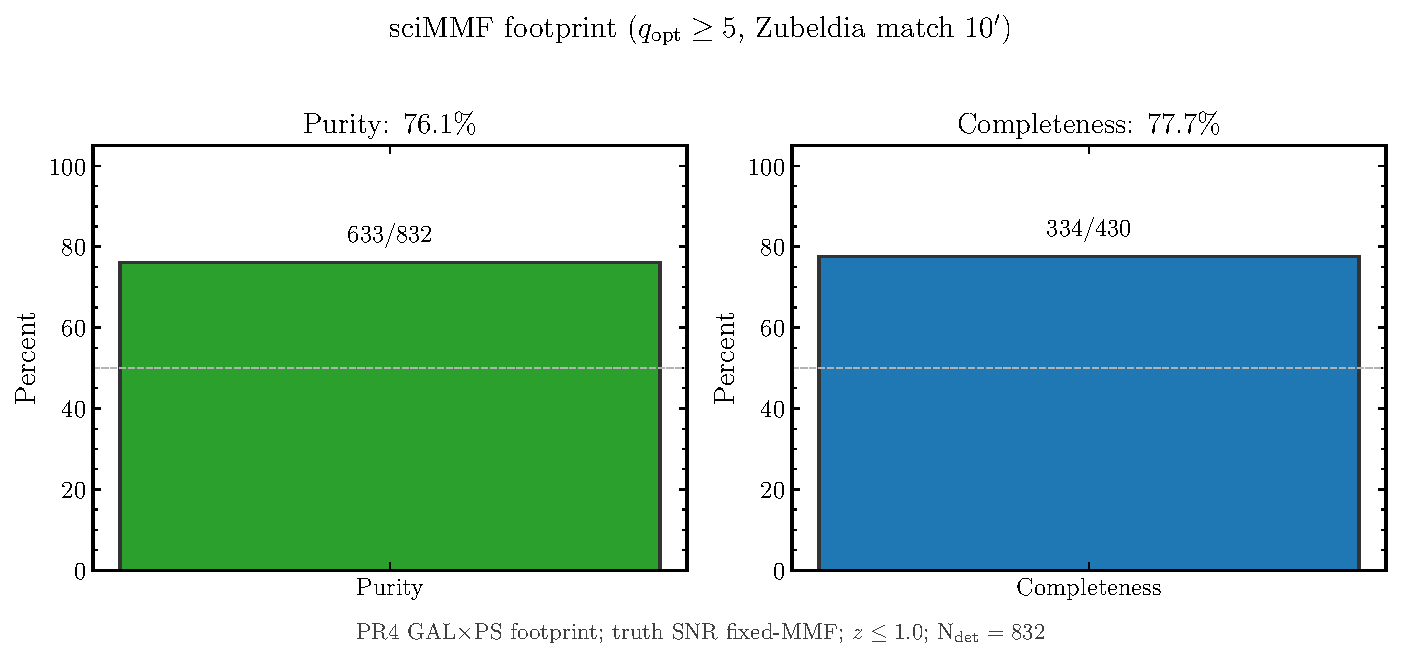
\includegraphics[width=0.49\textwidth]{szifi_footprint_scimmf_benchmark_szifi.pdf}
  \caption{Purity and completeness for footprint catalogues at $\qopt\ge 5$:
    iMMF (left; $333/430$ detectable truths found) and sciMMF (right;
    $334/430$).}
  \label{fig:szifi-bench}
\end{figure}

\begin{figure}[htbp]
  \centering
  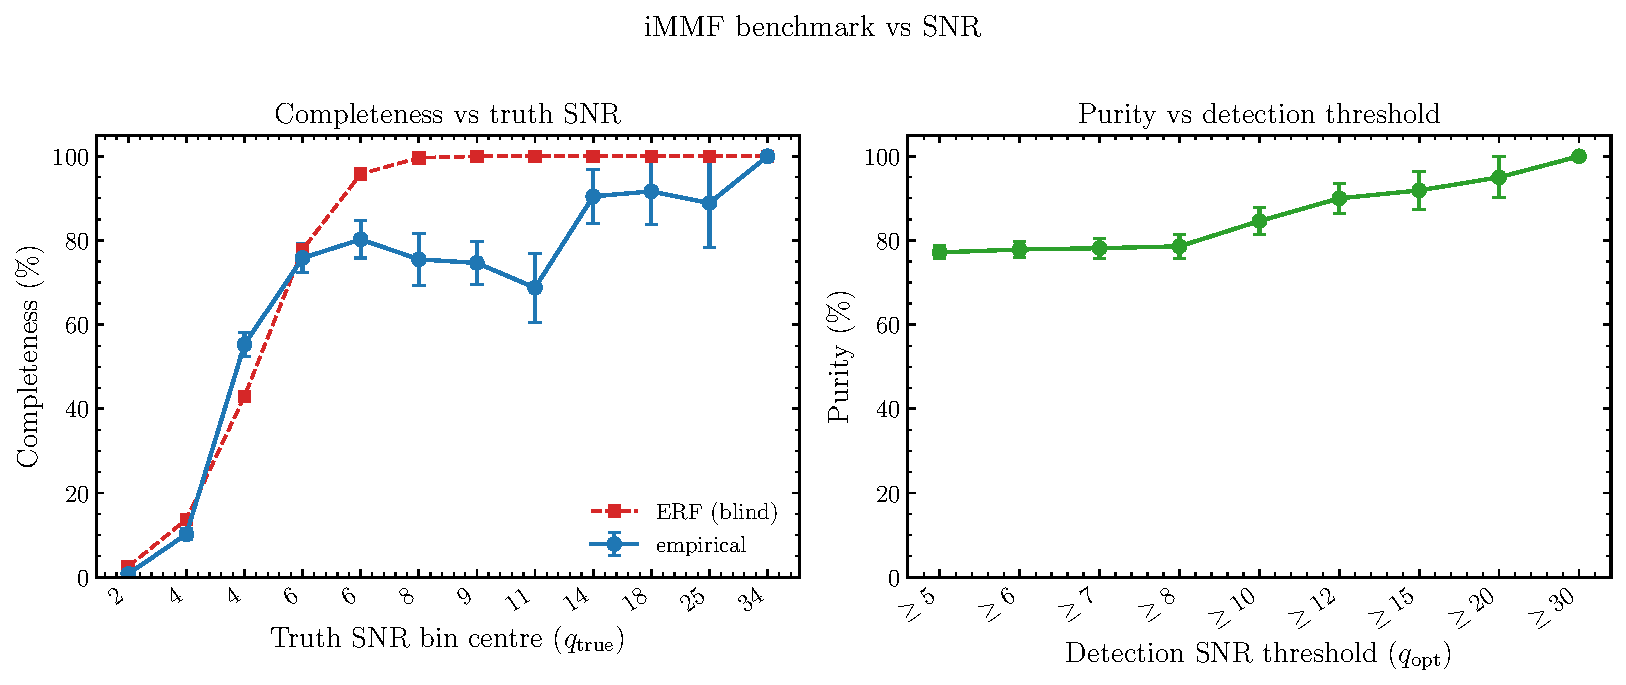
\includegraphics[width=0.49\textwidth]{szifi_footprint_immf_benchmark_snr_bins_szifi.pdf}
  \hfill
  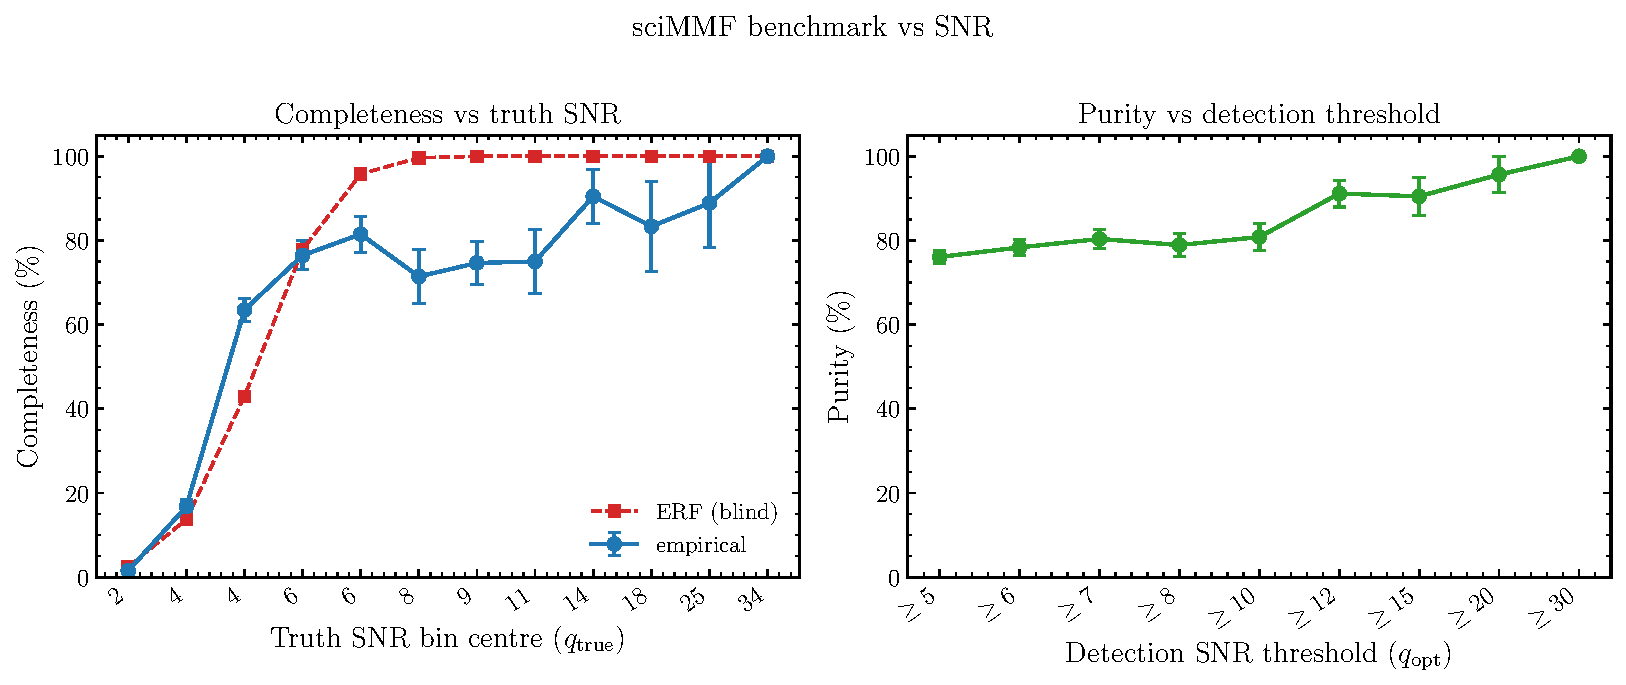
\includegraphics[width=0.49\textwidth]{szifi_footprint_scimmf_benchmark_snr_bins_szifi.pdf}
  \caption{Completeness versus truth SNR bin and purity versus detection SNR
    threshold for iMMF (left) and sciMMF (right).}
  \label{fig:szifi-snr}
\end{figure}

\begin{figure}[htbp]
  \centering
  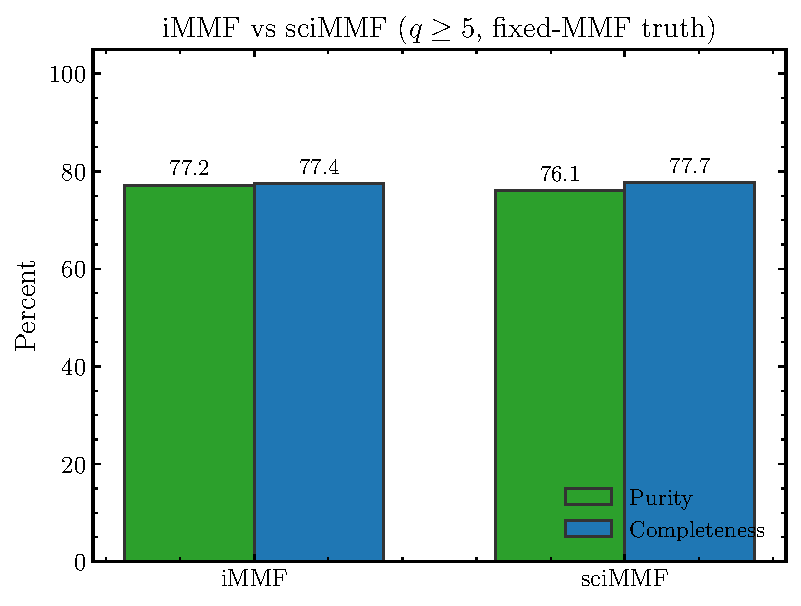
\includegraphics[width=0.85\textwidth]{szifi_footprint_purity_immf_scimmf.pdf}
  \caption{Purity and completeness for iMMF and sciMMF on the same footprint and
    truth definition.}
  \label{fig:szifi-compare}
\end{figure}

% Flush Results floats before Discussion
\clearpage

%==============================================================================
\section{Discussion and conclusions}
\label{sec:conclusions}
%==============================================================================

We have constructed multi-frequency CMB skies from FLAMINGO lightcones and used
them to validate secondary-anisotropy statistics and to test ILC $y$ recovery and
matched-filter cluster finding under Planck-like noise and masking. Our main
conclusions are as follows.

\begin{enumerate}
  \item \textbf{A four-component extragalactic sky is sufficient for controlled
    Planck-like SZ tests.} Lensed primary CMB, non-relativistic tSZ, kSZ and CIB,
    with common lightcone rotations, capture the secondaries and foregrounds most
    relevant to SZ science while excluding Galactic emission and radio sources by
    design. The resulting isolation is appropriate for algorithm tests; it is not
    a claim of full sky realism at $545$--$857\GHz$.

  \item \textbf{Spectral conversions must be applied consistently.} The
    non-relativistic tSZ function $f(x)$, the kSZ relation
    $\Delta T=-T_{\mathrm{CMB}}b$, thermodynamic conversion of CIB intensity, and
    NPIPE unit conventions ($K_{\mathrm{CMB}}$ versus $\mathrm{MJy\,sr^{-1}}$)
    fully specify the multi-frequency model used here.

  \item \textbf{Native-resolution power spectra validate the maps.} CIB autos,
    frequency decorrelation, CIB$\times y$ and CIB$\times\kappa$ crosses, and
    $y$/kSZ/$\kappa$ autos recovered from the lightcone products are consistent
    with Yang et~al.\ (2026). Downstream ILC and matched-filter analyses therefore
    start from spectrally faithful skies.

  \item \textbf{ILC recovers large-scale $y$; mild CIB deprojection helps,
    multi-moment constraints do not.} HILC and NILC recover the truth $y$
    spectrum after $5'$ beam deconvolution. In an eight-way constrained-ILC
    suite, CIB-only deprojection raises mid-$\ell$ correlation
    ($\rho_{50\text{--}500}$: $0.654\to 0.671$) and transfer
    ($T_{\mathrm{mid}}$: $0.909\to 0.960$), whereas
    $\mathrm{CIB}+\delta\beta+\delta T$ more than doubles $\sigma_y$ and
    collapses the correlation with truth.

  \item \textbf{iMMF and sciMMF recover clusters with purity and completeness
    both near $77\%$.} At $\qopt\ge 5$ on a Planck-like footprint we find purity
    $\approx 77.2\%$ (iMMF; $564$ TP / $167$ FP) and $\approx 76.1\%$ (sciMMF;
    $633$ TP / $199$ FP), with completeness of fixed-MMF-detectable systems
    $\approx 77\%$ ($333/430$ and $334/430$ truths found). Sky maps of detections
    and TP/FP classifications show that high-$q$ systems sit on bright $y$ peaks
    while residual false positives include threshold noise and boundary matches.
    sciMMF yields a larger catalogue at similar purity.

  \item \textbf{Limitations.} Results use a single lightcone, a single NPIPE
    realisation for cluster finding (split A), Gaussian beams, and no radio
    sources or Galactic dust. Completeness depends on the truth SNR definition.
    Multi-split cosmology analyses and fully redshift-matched halo comparisons
    remain for future work.
\end{enumerate}

In summary, FLAMINGO-based multi-frequency skies provide a rigorous laboratory
for millimetre component separation and cluster finding under realistic Planck
noise and masking, with component-level truth that is unavailable in flight data.

\clearpage

\begin{thebibliography}{99}

\bibitem[Lewis \& Challinor(2006)]{Lewis:2000camb}
A.~Lewis and A.~Challinor,
``Weak gravitational lensing of the CMB,''
Phys.\ Rep.\ \textbf{429}, 1 (2006).

\bibitem[McCarthy \& Hill(2024)]{McCarthyHill:2024}
F.~McCarthy and J.~C.~Hill,
``Component-separated, CIB-cleaned thermal Sunyaev--Zel'dovich maps from
\textit{Planck} PR4 data with a flexible public needlet ILC pipeline,''
Phys.\ Rev.\ D \textbf{109}, 023528 (2024),
arXiv:2307.01043.

\bibitem[Planck Collaboration(2020)]{Planck:2020npipe}
Planck Collaboration,
``Planck intermediate results. LVII. Joint Planck LFI and HFI data processing,''
Astron.\ Astrophys.\ \textbf{643}, A42 (2020),
arXiv:2007.04997.

\bibitem[Yang et~al.(2026)]{Yang:2026flamingo}
T.~Yang et~al.,
``Self-consistent secondary cosmic microwave background anisotropies and
extragalactic foregrounds in the FLAMINGO simulations,''
arXiv:2512.09891 (2026).

\bibitem[Zubeldia et~al.(2023a)]{Zubeldia:2023a}
\'I.~Zubeldia, A.~Rotti, J.~Chluba and R.~Battye,
``The multipole space of multi-frequency matched filters for the detection of
galaxy clusters,''
Mon.\ Not.\ R.\ Astron.\ Soc.\ \textbf{522}, 4766 (2023),
arXiv:2204.13780.

\bibitem[Zubeldia et~al.(2023b)]{Zubeldia:2023b}
\'I.~Zubeldia, A.~Rotti, J.~Chluba and R.~Battye,
``Spectral deprojection of the thermal Sunyaev--Zel'dovich effect,''
Mon.\ Not.\ R.\ Astron.\ Soc.\ \textbf{522}, 5123 (2023),
arXiv:2212.07410.

\end{thebibliography}

\end{document}
